\chapter[Fundamentação Teórica]{Fundamentação Teórica}
\label{cap-fundamentacao_teorica}

\section{O Empreendedorismo}
\label{section:o_empreendedorismo}

Segundo \citeonline{McCall2000}, a palavra Empreendedor tem sua origem na França, ainda no século XVII, e tem como um dos seus significados aquele encarregado por executar um determinado trabalho para os outros. Ele também diz que o termo também tem relação com a palavra francesa ``Entreprenant'', usada para descrever uma pessoa forte e audacioso e como alguém que constrói uma visão.

\citeonline{Brown2013} diz que a primeira citação documentada ao termo foi criada por Richard Cantillon (1697-1734) em seu livro ``Sobre a Natureza do Comércio em Geral''\footciteref{James1953}, o qual define Empreendedorismo como o processo de assumir risco ao adquirir bens a um determinado preço para vendê-los por um valor incerto no futuro, concretizando o lucro ou o prejuízo. Pelo seu contexto histórico enquanto em vida, um autor do século XVIII, muitas das suas visões eram baseadas nos negócios da época e para ele o empreendedor era prioritariamente como um fornecedor de produtos e serviços, e por isso menciona como empreendedores profissionais das mais diversas profissões, como proprietários de minas e teatros, fazendeiros, atacadistas de lã e grãos, mercadores, padeiros, artesãos, carpinteiros, pintores, médicos, advogados e até mesmo cervejeiros. 

Alguns séculos depois, \citeonline{Schumpeter1934} escreveu que o Empreendedorismo é o principal mecânismo no processo de desenvolvimento econômico e com ele é impossível não abalar o status quo do sistema econômico, ele defende que é graças as ações inovadoras dos empreendedores que nossos sistemas evoluem e são renovados. Outros autores como \citeonline{Holcombe1998, Acs2006} também defendem o Empreendedorismo como um impulsionador da economia. \citeonline{McClelland1961} sugere que o Empreendedorismo é responsável pelo avanço da civilicação por instigar o espiríto empreendedor na sociedade, de forma a permitir que explorem e inovem com a combinação dos recursos disponíveis.

\citeonline{Stevenson1985} diz que Administradores costumam definir ``Empreendedorismo'' com termos como inovador, flexível, dinâmico, tomador de risco e orientado ao crescimento. A mídia, ao promover o sucesso de grandes corporações como a Apple, o relacionam com a criação e expansão de novas empresas. No artigo ``The Heart of Entrepreneurship'' ele defende que o Empreendedorismo está muito mais relacionado à oportunidades do que aos recursos. \citeonline{Acs2006} diz que históricamente o termo é usado como referência à posse e gestão de uma empresa.

Para \citeonline{Dornelas2005} Empreendedorismo é o envolvimento de pessoas e processos que, em conjunto, levam à transformação de ideias em oportunidades. E a perfeita implementação destas oportunidades leva à criação de negócios de sucesso.

\citeonline{Drucker2006}, uma das maiores referências da área de Administração, define Empreendedorismo como uma disciplina que pode ser aprendida e praticada e como um processo para criação e gestão da inovação. 

Para ele inovar é criar uma nova forma de entregar um valor novo para os seus consumidores com os recursos que o empreendedor tem disponível. Com base nessas premissas e na visão de Drucker, se uma pessoa decide criar uma nova, porém tradicional, padaria como diversas outras em uma área residencial qualquer, ela provavelmente não será inovadora, e consequentemente seus criadores não estarão empreendendo, mas replicando modelos de negócios com processos e recursos já conhecidos e maturados por outras pessoas, talvez esses, sim, empreendedores. Ou seja, criar uma nova empresa não necessariamente significa estar empreendendo. Para isso é necessário inovar. 

Essa visão de Drucker pode ser facilmente relacionada a visão de \citeonline{Thurik2004}, que faz distinção entre empresas empreendedoras e empresas pequenas, com foco em pequenos negócios. \citeonline{Carland1984} define como ponto chave para essa distinção o crescimento expoencial das empresas empreendedoras, enquanto as pequenas empresas tendem a se manter pequenas por toda a sua vida, mesmo que demonstrem algum pequeno crescimento. 

No mesmo artigo \citeonline{Carland1984} define que pequenos negócios são quaisquer negócios independentes e não dominantes em seus mercados que não se envolvam com nenhuma prática de marketing ou inovação enquanto empresas empreendedoras são quaisquer negócios que se enquadrem em pelo menos uma das categorias de comportamento de \citeonline{Schumpeter1934} (novos produtos ou melhoria de produtos existentes, novos métodos de produção, abertura de novos mercados, domínio de novas fontes de fornecimento e matéria-prima ou reorganização industrial). Para ele, uma empresa empreendedora deve ser inovadora, lucrativa e estar em constante expansão.

Quando os irmãos McDonald\footciteref{RichardMcDonald2016} decidiram aplicar conceitos e técnicas de gestão de negócios e de produção com a padronização de seus sanduíches e desenvolvimento de processos de produção padronizados eles inovaram. Conseguiram maximizar os retornos com seus recursos, criaram um novo mercado, definiram um novo padrão para a indústria de alimentos e atualmente alimentam mais de 68 milhões de consumidores em cerca de 36 mil restaurantes em 119 países\footciteref{McDonald2016}, para uma empresa que iniciou operação em 1940 com um único restaurante esse foi um crescimento muito acelerado.

\citeonline{Birley1986} define empresas empreendedoras como orgânicas e com um grande enfoque nos relacionamentos ao invés de mecânicas e burocrácias, essa características são muito presentes nas Startups.

\citeonline{McCall2000} relata que o ``The Entrepreneurship Center at Miami University of Ohio'' define Empreendedorismo como o processo de identificar, desenvolver e dar vida a uma visão. Essa visão pode ser uma idéia inovadora, uma oportunidade ou uma forma melhor de realizar alguma atividade ou serviço.

Para \citeonline{Schumpeter1934} o Empreendedorismo é capaz de fornecer um excelente mecanismo de mobilidade social, para que o indivíduo seja capaz de levar sua família para um status social mais elevado. \citeonline{Byers2014} já defende que o Empreendedorismo envolve a criação de um novo empreendimento que sirva a sociedade e crie mudanças positivas, algo muito além da criação de uma empresa e da geração de riquezas. 

Para \citeonline{Hill1994} Empreendedorismo é o processo que causa mudanças no sistema econômico através de inovações de indíviduos que criaram ou aproveitaram oportunidades que criem valor tanto para eles próprios como também para a sociedade.

Para \citeonline{Wallevik2016}, não há um senso comum do significado e do histórico do termo ``Empreendedorismo'', os conceitos variam de acordo com o contexto estudado podendo englobar diversos cenários distintos como a criação e expansão de grandes empresas mas também envolvendo atividades de impacto social, no campo, em pequenos negócios sociais e até mesmo como empregados de grandes corporações, sejam elas privadas ou públicas. 

\citeonline{Paternoster2014} diz que o Empreendedorismo Moderno, com foco nos mercados de tecnologia, foi impulsionado pelo advento dos mercados de consumo pela internet na década de 90, ao fácil acesso à esses mercados e ao baixo custo de distribuição.

\section{O Empreendedor}
\label{section:o_empreendedor}

Assim como em relação ao \ref{section:o_empreendedorismo}, ainda não há um consenso em relação ao significado do termo ``Empreendedor'' na Academia, como citado por \citeonline{Fernald2005} os autores sugerem uma série de critérios que envolvem criatividade, inovação, características pessoais e até mesmo aparência e estilo. O mesmo autor classifica Empreendedores como pessoas que tiram vantagens e conseguem obter valor das oportunidades que surgem.

\citeonline{Stevenson1985} diz que Empreendedores não são apenas seres oportunistas mas também criativos e inovadoras. \citeonline{Drucker2006} relata que estão sempre em busca por mudanças, respondem à ela e aproveitam a oportunidade.

Para \citeonline{Byers2014} Empreendedores são pessoas que identificam soluções entre problemas, possibilidades entre necessidades e oportunidades entre desafios, de forma a criar ótimos empreendimentos que demonstram competência, liderança e longetividade. 

\citeonline{Schumpeter1934} traz atenção para a importância da intuição e coragem do Empreendedor na sua busca pelo sucesso, especialmente em campos em que não haja domínio do problema ou quando o planejamento precisa ser alterado. \citeonline{Schackle1982} define o Empreendedor como um fazedor de histórias, mas seu guia para construí-las é sua intuição e capacidade de julgamento das possibilidades.

\citeonline{Acs2006} defende um sentido mais amplo ao fazer referência ao comportamento empreendedor de estar sempre em busca de uma nova oportunidade para Empreender, mas não necessariamente com a criação de um novo negócio. \citeonline{Acs2016} relata que aqueles que estão com economias movidas pela inovação terão mais chance de afetar seus Ecossistemas pelo seu crescimento.

Para \citeonline{Bygrave1991} o Empreendedor é aquele que persegue uma oportunidade e cria uma organização para domina-la.

Na mesma linha explorada por \citeonline{Thurik2004, Carland1984}, mencionados na seção \ref{section:o_empreendedorismo}, em que empreendimentos são divididos entre empreendedores ou pequenos negócios \citeonline{Spring2014} faz diferenciações entre os donos de pequenos negócios e os Empreendedores. Para ela, empreendedores são aqueles com grandes sonhos e ideias e motivados pela incerteza e o risco da criação de um novo empreendimento, além de serem os que trabalham com foco no futuro e na escala. A mesma autora define donos de pequenos negócios como pessoas que optam por abordagens conservadoras e calculadas e com um grande apego emocional aos seus negócios.

Essa visão do Empreendedor motivado pelo risco e pela incerteza, oportunistas, inovadores, criativos, líderes e solucionadores de problema são essenciais para o sucesso de uma Startup.

\section{A Startup}
\label{section:as_startups}

Não se sabe ao certo quem criou o termo ``Startup'', \citeonline{Miranda2015, Brigidi2009} relatam que o termo tem sido usado de maneira ampla em diversos contexto e sem uma definição clara. \citeonline{Gitahy2010} descreve o termo como um sinônimo para criação de novas empresas e que, embora muito comum nos Estados Unidos da América há muitos anos, começou a ser usado no Brasil após a bolha da internet\footciteref{BolhaDaInternet}.

Com o advento dos dispositivos móveis e de recursos de internet cada vez mais acessíveis, \citeonline{Paternoster2014} defende que estamos em uma nova bolha, a Bolha das Startups, por conta da grande ploriferação de novas empresas de tecnologia.

\citeonline{Blank2014} enfatiza que uma Startup não é uma versão menor de uma grande companhia e a define como uma organização temporária em busca de um modelo de negócio escalável, recorrente e lucrativo. O motivo dessa definição está esclarecido na seção sobre \ref{section:o_ciclo_de_vida}. \citeonline{Blank2010} também  diz que existem seis tipos de Startups: 

\begin{description}
	\item [Estilo de Vida:] aquelas que seus criadores trabalham exclusivamente motivados pela paixão que possuem por determinada tecnologia ou produto.

	\item [Pequenos Negócios:] Blank também considera como Startups os pequenos e tradicionais negócios como salões de beleza, mercados, etc.

	\item [Escaláveis:] Startups que crescem rapidamente em níveis globais como aconteceu com o Google e o Facebook e seus fundadores são motivados pela possibilidade de faturar milhões com sua venda ou abertura de capital.

	\item [Compráveis:] aquelas que são criadas já com o objetivo de serem adquiridas e incorporadas por Grandes Empresas.

	\item [Grandes Empresas:] já estão estabelecidas, geralmente crescem por meio de processos de inovação sustentáveis, aquisição de outras Startups, etc. Atualmente Google e Facebook são exemplos de Grandes Empresas.

	\item [Sociais:] Startups que tem como seu maior objetivo criar um mundo melhor e não acumular riqueza. Podem ter fins lucrativos, não ter fins lucrativos ou seguirem um modelo misto.
\end{description}

Para \citeonline{Ries2011}, uma Startup é uma instituição humana projetada para criar novos produtos e serviços sob condições de extrema incerteza. Ries não fala sobre tamanho, setor ou indústria e afirma que Startups podem co-existir até mesmo dentro de grandes corporações. Para ele, o maior objetivo de uma Startup é descobrir qual o produto certo que os consumidores queiram e estejam dispostos a comprar, e/ou usar, o mais rápido possível. 

\begin{quote}
As startups utilizam muitos tipos de inovação: descobertas científicas originais, um novo uso para uma tecnologia existente, criação de um novo modelo de negócios que libera um valor que estava oculto, ou a simples disponibilização do produto ou serviço num novo local ou para um conjunto de clientes anteriormente mal atendidos. Em todos esses casos, a inovação é o cerne do sucesso da empresa. \cite{Ries2011}
\end{quote}

\citeonline{Graham2012} diz que o único fator essencial para que uma organização seja classificada como uma Startuup é o seu crescimento, para ele qualquer outro fator nada mais é do que um reflexo deste e que não é necessário que o produto seja relacionado a tecnologia ou receba investimento para que seja uma Startup.

\citeonline{Sutton2000} mapeou algumas características sobre Startups e para ele sua característica mais básica é ser nova e inexperiente quando comparada com organizações estabelecidas e maduras. Ele também as caracteriza como organizações sensíveis à diversos influenciadores (investidores, clientes, parceiros e concorrentes) que trabalham com poucos recursos e geralmente acompanham novas tendências de tecnologia e mercado. \citeonline{Paternoster2014} diz que Startups muitas vezes precisam utilizar novas tecnologias, ferramentas e técnicas para conseguirem desenvolver produtos tecnologiamente inovadores. Esse cenário condiz com o mapeamento realizado por \citeonline{Polovets2014} em que a maior parte das Startups registradas no AngelList\footciteref{AngelList} utilizam tecnologias modernas como Javascript, Node.js, Ruby, Ruby on Rails, Python e HTML5 e hospedam seus softwares em grandes infraestruturas escaláveis como Amazon Web Services\footciteref{AmazonWebServices} e Heroku\footciteref{Heroku}.

Em uma entrevista documentada por \citeonline{Robehmed2013} o Empreendedor Neil Blumenthal definiu Startup como uma companhia trabalhando para resolver um problema o qual a solução não é óbvia e o sucesso incerto. Na rede social de perguntas e respostas Quora\footciteref{Quora} o Empreendedor Dave McClure definiu Startups como empresas confusas em relação ao que é o seu produto, quem é o seu cliente e como monetizar com sua solução e que logo após obter resposta para essas três perguntas elas deixam de ser uma Startup e se tornam negócios reais.

Alguns especialistas tentam definir métricas para traçar o momento em que esses novos empreendimentos deixem de ser classificados como Startups. \citeonline{Wilhelm2014} sugere a regra dos ``50, 100 ou 500'': US\$50 milhões em vendas nos últimos 12 meses, 100 ou mais empregados e valor de mercado avaliado em mais de US\$500 milhões.   

No primeiro Edital do Programa Startups Brasilia\footciteref{StartupBrasilia2015} do Governo de Brasília para subvenção de projetos de inovação tecnológica a Fundação de Apoio à Pesquisa do Distrito Federal define Startups como empresas cujo faturamento anual seja inferior R\$ 3,6 milhões e possuam menos de quatro anos de existência. 

A Fundação Carlos Chaga de Amparo à Pesquisa do Estado do Rio de Janeiro(FAPERJ) com o programa Startup Rio\footciteref{StartupRio2015} classifica como Startups as Micro Empresas com potencial de crescer rapidamente e iniciar operação em outros estados e países em poucos meses de atividade. Por esse motivo defendem que o termo é comumente utilizado para Micro Empresas de base tecnológica, por não possuirem tantas barreiras logísticas que impeçam uma expansão tão grande e tão rápido.

A Financiadora de Projetos e Pesquisa(FINEP)\footciteref{Finep2016}, outra entidade pública do Brasil para fomento à inovação, define Startup como uma Empresa Nascente de Base Tecnológica sujeita a frequentes mudanças e que tem como sua maior sustenção a inovação. Para eles, Startups possuem uma estrutura empresarial(uma ``quase empresa'', como definido em seu Glossário\footciteref{GlossarioFinep}), não possuem posição definida no mercado e estão em busca por oportunidades com produtos de alto valor agregado.

\section{O Ciclo de Vida}
\label{section:o_ciclo_de_vida}

\citeonline{Pires2012} diz que o o ciclo de vida de uma Startup é a busca pelo seu modelo de negócios. \citeonline{Blank2014} divide o Ciclo de Vida de uma Startup em três níveis, como representado pelas Figura XX e Figura XX.

\begin{figure}[!htb]
\centering
\includegraphics[width=11cm,angle=0]{figuras/ciclo_de_vida_steve_blank}
\caption{Representação do Ciclo de Vida de uma Startup Escalável por \cite{Blank2014}}
\label{Rotulo}
\end{figure}

\begin{figure}[!htb]
\centering
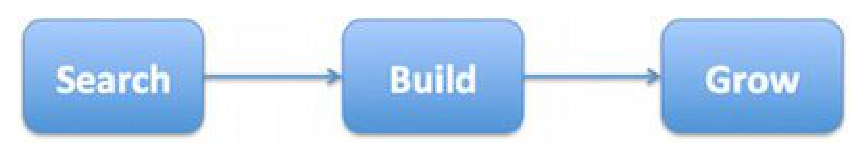
\includegraphics[width=11cm,angle=0]{figuras/ciclo_de_vida_steve_blank02}
\caption{Representação do Ciclo de Vida de uma Startup por \cite{Blank2015}}
\label{Rotulo}
\end{figure}

No primeiro nível, o objetivo da Startup é identificar e validar um modelo de negócios que seja repetível e escalável, em outras palavras: descobrir o que você vai construir e quem vai compra-lo. \citeonline{Blank2014} diz que é normal que sejam necessárias várias iterações e ``pivotagens'' até encontrar um bom produto e um mercado que possa ser atacado. Nesse nível, as Startups costumam ser pequenas e não muito estruturadas, elas ainda estão imersas em um ambiente de extrema incerteza e um cenário de tentativas e erros e por esse motivo é onde a maior parte morre. Na Figura XX \citeonline{Byers2014} apresenta um modelo de como combinar os interesses e paixões dos empreendedores com suas capacidades e oportunidades do mercado com o objetivo de encontrar o ``pote de ouro'', encontrar o que será o seu produto.

\begin{figure}[!htb]
\centering
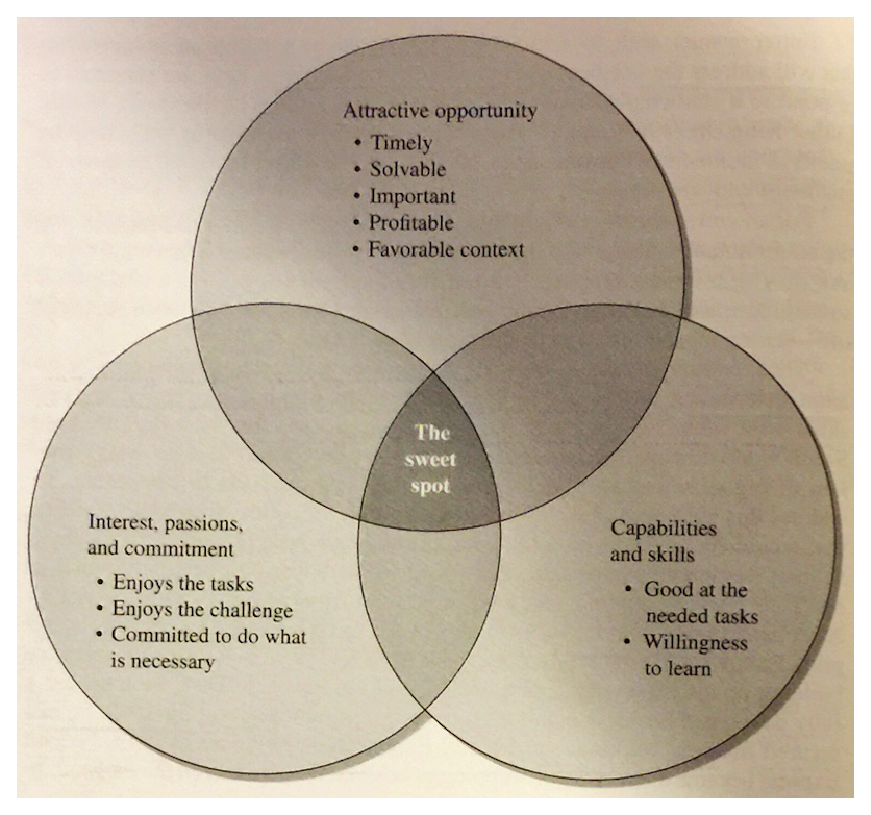
\includegraphics[width=11cm,angle=0]{figuras/the_sweet_spot_byers}
\caption{Representação de como encontrar uma oportunidade por \cite{Byers2014}}
\label{Rotulo}
\end{figure}

Durante o segundo nível, a Startup se encontra em uma fase de transição para se tornar uma empresa que precisa escalar e crescer de forma sustentável. O maior objetivo aqui é atingir um fluxo de caixa positivo, geralmente nesse nível a Startup começa a se tornar uma grande organização, com muitos funcionários, e processos e hierarquias precisam começar a ser definidos para evitar o caos, o crescimento desordenado e garantir que a cultura da empresa será mantida. Segundo Blank, há casos em que as Startups possam ter até 700 funcionários e ainda estarem nesse nível.

No terceiro e último nível, a empresa já atingiu líquidez e está crescendo com a implementação contínua dos processos que foram definidos no nível anterior. É comum que aqui o capital da empresa já tenha sido aberto ou tenha sido vendida. 

\citeonline{Ries2011}, um dos alunos mais ilustres que Steve Blank já teve, trás grande enfâse para a importância que falhar possui no desenvolvimento da sua Startup, e mais precisamente falhar rápido. Seu ciclo de vida tem como objetivo acelerar o caminho da Startup, seja para o sucesso ou para o completo fracasso, caso a equipe chegue a conclusão de que não são capazes de encontrar um modelo de negócios sustentável e repetível. O quanto antes o Empreendedor encontrar o caminho certo, maiores as chances de sua Startup sobreviver. A raiz desse ciclo está representada na figura XX.

A partir das ideias, ele e Blank defendem que o Empreendedor deve construir um Mínimo Produto Viável(ou MVP, como é conhecido pela abreviação do termo na língua inglesa) que corresponda ao menor, ou mais simples, pedaço de produto para que seja possível que a proposta seja validada e lições sejam aprendidas com base no feedback dos usuários. Em seu livro Ries diz que qualquer trabalho adicional além do que é necessário para que a equipe comece a aprender é desperdício, não importa o quão importantes esses recursos extras possam parecer. Para que o aprendizado seja possível, dados precisam ser coletados e medidos. Afinal, como diz o ditado que alguns atribuem à Peter Drucker: ``O que não pode ser medido não pode ser melhorado''. 

\begin{figure}[!htb]
\centering
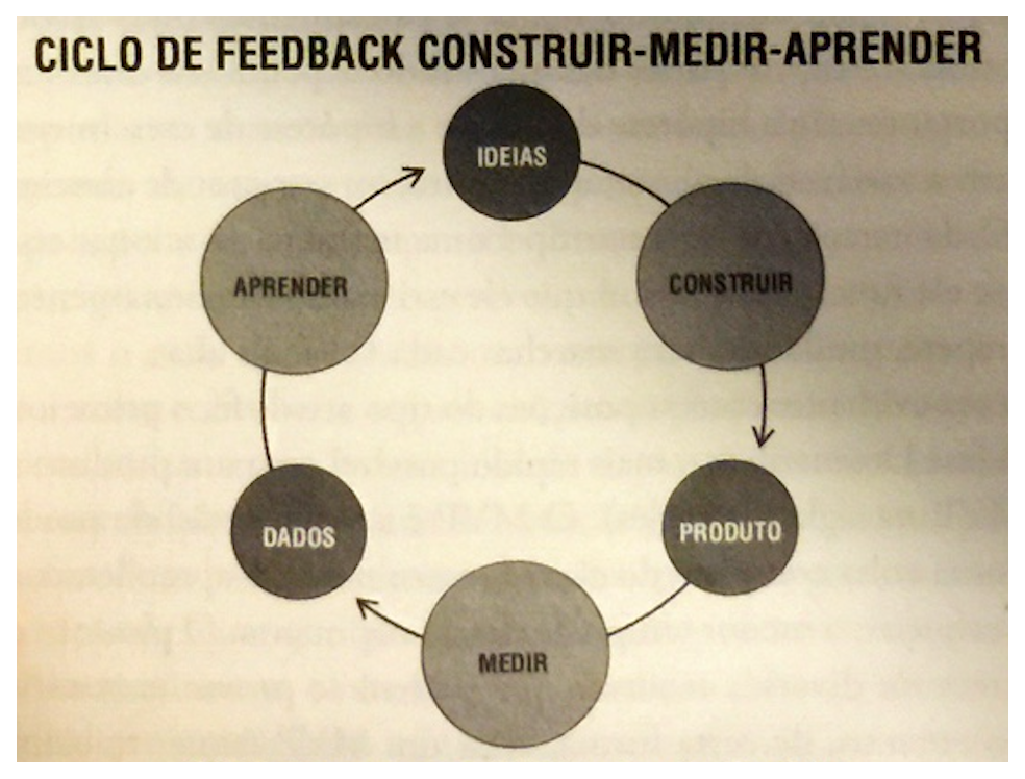
\includegraphics[width=11cm,angle=0]{figuras/ciclo_de_vida_eric_ries}
\caption{Representação do Ciclo de Vida de uma Startup por \cite{Ries2011}}
\label{Rotulo}
\end{figure}

Uma das frases mais emblemáticas do livro ``Startup Enxuta'' é que se empreendedor não pode falhar, então não poderá aprender. E isso se torna claro com esse ciclo de vida proposto por \citeonline{Ries2011}. Quanto maior o número de iterações, maior a quantidade de falhas e consequentemente maior será o aprendizado. Para ele, esse modelo de Costruir, Medir e Aprender com base em loops iterativos e feedbacks constantes

Para \citeonline{Graham2012} o ciclo de vida de uma Startup de sucesso geralmente possui três fases: um período inicial de pequeno ou nenhum crescimento enquanto a Startup ainda está tentando descobrir qual o seu propósito e produto, uma fase intermediária com um rápido crescimento após a descoberta de qual o produto desejado pelas pessoas e como vendê-lo e, por fim, a Startup se torna uma Grande Empresa, cheia de processos e com uma redução da taxa de crescimento, mas um grande domínio do mercado.

\citeonline{Polgar2015} relata que Graham também criou um diagrama da curva de crescimento de uma Startup, representado na Figura XX. Esse ciclo apresenta um momento muito interessante que quase todas as Startups precisam superar: logo após o ápice de entusiasmo e energia dos Empreendedores após ter uma ideia e começar a sua implementação eles encontram a fase que é conhecida como ``Trough of Sorrow'', ou o Vale da morte, em que a equipe se depara com a realidade e começa a enfrentar muitas das dificuldades inerentes da criação de uma Startup. Esse será um momento de muita experimentação, de muitas falhas, de muitas ``pivotagens'' e de muitos aprendizados, até que a equipe encontre um produto que uma determinada fatia de mercado esteja disposta a comprar, nesse momento a Startup volta a crescer e começa a escalar, mas também é o momento em que a maior parte irá morrer, como o nome sugere.

\begin{figure}[!htb]
\centering
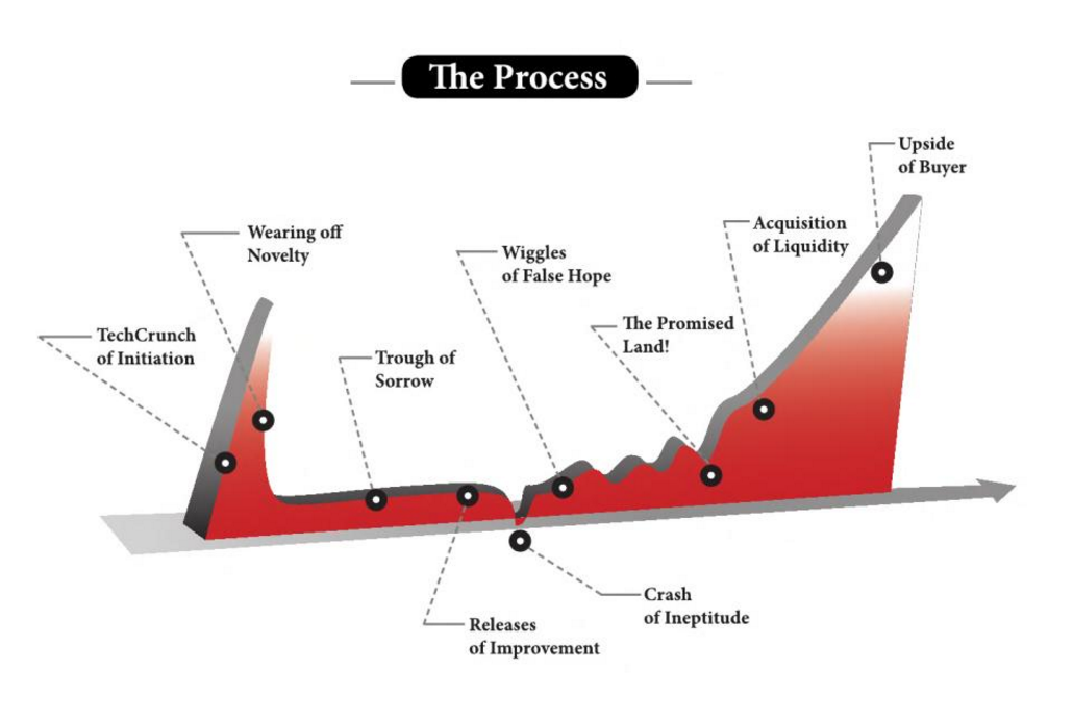
\includegraphics[width=11cm,angle=0]{figuras/startup_curve_by_graham}
\caption{Curva de crescimento de uma Startup por Paul Graham, representado por \cite{Polgar2015}}
\label{Rotulo}
\end{figure}

\citeonline{Crowne2002} descreve três fases no ciclo de vida de uma Startup: a primeira, descrita como Startup, a fase de Estabilização e a fase de Crescimento.  A primeira fase é marcada pelo período em que o produto ainda é um conceito até a sua primeira venda concreteizada. A segunda fase acontece até o momento em que o produto e os processos da Startup são estáveis o suficiente para que a entrada de novos clientes não façam a organização perder o controle de si mesmo. A última tem seu início com o começo da venda dos produtos de uma Startup em escala e se mantém até que a Startup alcance o nível de uma organização.

\citeonline{marmer2011startup}, por meio do Startup Genome, organização sem fins lucrativos que realiza análises de Ecossistemas de Startups em todo o mundo entrevistou cerca de 11 mil Empreendedores em 40 Ecossistemas e dividiu o ciclo de vida de uma Startup em seis estágios: a Descoberta, a Validação, a Eficiência, a Escala, a Sustentabilidade e a fase de Conservação. 

Como um dos resultados dessa pesquisa descobriram a grande importância que esse ciclo possui nas chances de sucesso de uma Startup, de forma que aquelas que cresceram de forma muito acelerada e inconsistente, sem respeitar o desenvolvimento de todas as fases do ciclo e suas capacidades, obtiveram resultados muito inferiores, como representado na figura XX. 

\begin{figure}[!htb]
\centering
\includegraphics[width=11cm,angle=0]{figuras/valuation_ao_escalar}
\caption{Representação de como o valor de uma Startup que recebeu investimento mas se desenvolveu de forma consistente cresce muito mais do que o de uma Startup que não respeitou o seu ciclo de vida, por \cite{marmer2011startup}}
\label{Rotulo}
\end{figure}

Também verificaram que cerca de 74\% das Startups que fizeram parte da pesquisa e cresceram de forma prematura falharam, gastaram cerca de 2,3 vezes mais do que a média com aquisição de clientes, nenhuma atingiu a marca de 100 mil usuários e 93\% nunca atingiram 100 mil dólares em vendas mensais. No artigo citado vários outros indicadores comparativos e fatores que caracterizam um crescimento inconsistente são apresentados.

\section{O dinâmico mercado das Startups}
\label{section:o_dinamico_mercado_das_startups}

\citeonline{James1953} fez uma análise que demonstra que o valor intríseco de um determinado produto, o seu valor de venda, está associado ao custo de oportunidade e não ao seu custo de produção. Dessa forma ele mostra como a economia poderia ser auto-regulada, visto que os empreendedores precisam respeitar os sinais do mercado para determinar o valor de um produto e essa é, para ele, a base do empreendedorismo e se mostra muito presente no mundo mesmo após 300 anos, principalmente entre algumas Startups e seu altíssimo valor de mercado mesmo quando ainda não há faturamento, como relatado por \citeonline{Luckerson2013}.

shumpeter argued that anyone seeking profits must innovate

Segundo Grahan (2012), é importante observar que o grande potencial de
escalabilidade pressupõe que haja um grande mercado disposto a querer usar o produto
ou serviço oferecido. Dessa forma, é necessário oferecer algo novo ao mercado.

Considerando que, se você quer começar uma
startup, você provavelmente vai ter que pensar em
algo bastante novo. Uma startup tem que fazer algo
que possa oferecer a um grande mercado, e as idéias
desse tipo são tão valiosas que todas as mais óbvias
já foram implementadas (...) Esse espaço de idéias
tem sido tão bem trabalhado que uma startup
geralmente tem que trabalhar em algo todo mundo
esqueceu.” (GRAHAN, 2012, p. 6)

Segundo a aceleradora Y Combinator 1
(2014), a taxa de crescimento de startups
de sucesso tendem a ser entre 5% a 7% por semana. Se o resultado ultrapassar 10% isso
significa um sucesso excepcional

Essa taxa de crescimento é medida a partir da receita. Contudo, se uma startup
não está sendo inicialmente monetizada, a segunda melhor mensuração, de acordo com
a Y Combinator, é a partir do número de usuário ativos. Essa é uma medição
considerada razoável porque as receitas futuras serão provavelmente um múltiplo
constante de usuários de usuários ativos. 

Segundo uma pesquisa realizada pelo Startup Genome Report Extra on
Premature Scaling2 (2014), no qual foram analisadas 3.200 empresas de alto
crescimento na área de web e mobile em 3 anos, 92% das startups falharam. Dessas,
74% falharam devido ao escalonamento prematuro.
Startups que mudam de plano uma ou duas vezes, adquirem 2,5 vezes mais
investimento mais dinheiro, possuem uma taxa de crescimento de usuário
3,6% melhor, e são 52% menos propensas a escalar prematuramente do que
startups que mudam de negócios mais de 2 vezes ou nenhuma vez.

. Equipes equilibradas, com um fundador técnico e um fundador da área de
negócios adquirem investimentos 30% maior, tem uma taxa de crescimento de
usuário 2,9 vezes maior e são 19% menos propensas a escalar prematuramente
do que as equipes somente técnicas ou somente da área de negócios

\section{O Ecossistema}
\label{section:ecossistemas_e_suas_pecas}

\citeonline{James1953} também diz que o crescimento econômico, a formação e o crescimento de cidades está diretamente ligado ao Empreendedorismo e as decisões que são tomadas por Empreendedores

While government agencies and educational institutions can create conditions favorable for entrepreneurship to take hold, it is up to individual organizations to foster the conditions that allow it to flourish the heart of entrepreneurship

schumpeter emphatizes the role of the entrepreneur as a prime cause of economic development,  thurik

\section{O Brasil}

“I am a huge believer in the idea that starting during a downturn is the best time to start,” says HBS Senior Lecturer Janet J. Kraus. “Opportunity costs are low, and if you’re able to turn a profit in a down market, then you will be very profitable when markets recover.”
